\documentclass[aspectratio=169,11pt]{beamer}
\usepackage[T1]{fontenc}
\usepackage{lmodern}
\usepackage{booktabs}
\usepackage{tikz}
\usetikzlibrary{arrows.meta,positioning,shapes.geometric}

\definecolor{wine}{HTML}{9F1724}
\definecolor{coral}{HTML}{E85D4A}
\definecolor{orange}{HTML}{D97A00}
\definecolor{cream}{HTML}{FFF4EE}
\definecolor{ink}{HTML}{33312E}
\definecolor{muted}{HTML}{756963}

\setbeamercolor{normal text}{fg=ink,bg=white}
\setbeamercolor{structure}{fg=wine}
\setbeamercolor{frametitle}{fg=white,bg=wine}
\setbeamercolor{block title}{fg=white,bg=wine}
\setbeamercolor{block body}{fg=ink,bg=cream}
\setbeamertemplate{navigation symbols}{}
\setbeamertemplate{itemize item}{\color{coral}$\blacktriangleright$}
\setbeamertemplate{itemize subitem}{\color{orange}$\bullet$}
\setbeamertemplate{frametitle}{\vspace{0.15cm}\hspace{0.25cm}\insertframetitle\strut\par}
\setbeamertemplate{footline}{%
  \leavevmode\hbox{%
  \begin{beamercolorbox}[wd=.82\paperwidth,ht=2.6ex,dp=1.1ex,leftskip=1em]{author in head/foot}%
    \color{muted}\insertshorttitle
  \end{beamercolorbox}%
  \begin{beamercolorbox}[wd=.18\paperwidth,ht=2.6ex,dp=1.1ex,center]{date in head/foot}%
    \color{wine}\insertframenumber/\inserttotalframenumber
  \end{beamercolorbox}}
}

\newcommand{\key}[1]{\textcolor{wine}{\textbf{#1}}}
\newcommand{\flowbox}[2][]{\node[draw=wine,rounded corners=3pt,fill=cream,minimum height=10mm,align=center,text width=25mm,#1] {#2};}

\title[MetricSpace]{Modern AutoCrit + MetricSpace}
\subtitle{An agentic clinical data-science tool for comparing eligibility criteria}
\author{Jonathan Ma \and Sijia Zhu \and Jiatong Gao}
\date{Project Proposal}

\begin{document}

\begin{frame}[plain]
  \begin{tikzpicture}[remember picture,overlay]
    \fill[cream] (current page.south west) rectangle (current page.north east);
    \fill[wine] (current page.north west) rectangle ([yshift=-1.15cm]current page.north east);
    \fill[coral] ([xshift=-1.2cm]current page.south east) circle (2.3cm);
  \end{tikzpicture}
  \vspace{1.0cm}
  {\usebeamerfont{title}\color{wine}\Huge\textbf{Modern AutoCrit + MetricSpace}\par}
  \vspace{0.3cm}
  {\Large An agentic clinical data-science tool for comparing eligibility criteria\par}
  \vspace{0.75cm}
  {\large Jonathan Ma \quad Sijia Zhu \quad Jiatong Gao\par}
  \vfill
  {\color{muted}Project proposal: clinical protocols, agentic AI, and validated decision support}
\end{frame}

\begin{frame}{Starting point: AutoCriteria}
\footnotesize
\begin{columns}[T,onlytextwidth]
  \column{0.54\textwidth}
  \begin{block}{Core idea}
    Use an LLM to convert free-text clinical-trial eligibility criteria into a more structured representation.
  \end{block}
  \vspace{0.15cm}
  \begin{itemize}
    \item Makes protocol prose easier to process computationally.
    \item Establishes the protocol-to-structure workflow.
    \item Motivates automated cleaning and normalization.
  \end{itemize}
  \column{0.42\textwidth}
  \begin{center}
  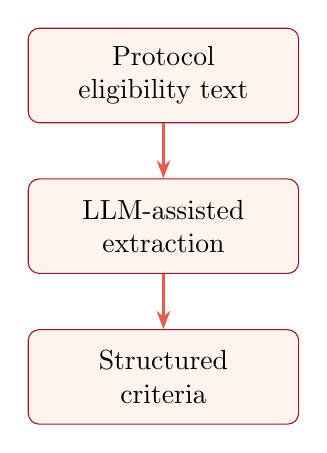
\begin{tikzpicture}[node distance=7mm]
    \node[draw=wine,rounded corners,fill=cream,text width=32mm,align=center,minimum height=12mm] (a) {Protocol\\eligibility text};
    \node[draw=wine,rounded corners,fill=cream,text width=32mm,align=center,minimum height=12mm,below=of a] (b) {LLM-assisted\\extraction};
    \node[draw=wine,rounded corners,fill=cream,text width=32mm,align=center,minimum height=12mm,below=of b] (c) {Structured\\criteria};
    \draw[-{Stealth},thick,coral] (a)--(b);
    \draw[-{Stealth},thick,coral] (b)--(c);
  \end{tikzpicture}
  \end{center}
\end{columns}
\end{frame}

\begin{frame}{Modern AutoCrit: work built on AutoCriteria}
\footnotesize
\begin{block}{From proof of concept to usable extraction tool}
AutoCriteria demonstrated LLM-based protocol structuring. Modern AutoCrit makes that workflow inspectable, reviewable, and reusable for downstream clinical data science.
\end{block}
\begin{columns}[T,onlytextwidth]
  \column{0.48\textwidth}
  \key{Engineering changes}
  \begin{itemize}
    \item Modular browser application instead of one long script.
    \item Input by NCT ID, pasted text, or full protocol PDF.
    \item ClinicalTrials.gov API v2 retrieval.
    \item Removed LangChain/LangGraph dependencies in favor of direct SDK calls and explicit workflow code.
    \item Fewer hidden abstractions make structured output, failures, and debugging easier to trace.
  \end{itemize}
  \column{0.48\textwidth}
  \key{More atomic, computable output}
  \begin{itemize}
    \item Separates compound sentences into independently comparable criteria.
    \item Domain, entity, comparator, value, unit, and interval.
    \item Negation, timing, repetition, qualifiers, and AND/OR logic.
    \item Preserves source evidence while normalizing terminology.
    \item Human review plus versioned JSON/CSV and Excel export.
  \end{itemize}
\end{columns}
\end{frame}

\begin{frame}{Why atomic extraction matters}
\small
\begin{block}{Source sentence}
``Exclude blood pressure $>145/95$ on two occasions within three months or a history of myocardial infarction.''
\end{block}
\begin{columns}[T,onlytextwidth]
  \column{0.48\textwidth}
  \key{Atomic criterion 1}
  \begin{itemize}
    \item Entity: blood pressure
    \item Comparator/value: $>145/95$
    \item Repetition: two occasions
    \item Time: within three months
    \item Logic: OR; type: exclusion
  \end{itemize}
  \column{0.48\textwidth}
  \key{Atomic criterion 2}
  \begin{itemize}
    \item Entity: myocardial infarction
    \item Value: present
    \item Temporal construct: history of
    \item Logic: OR; type: exclusion
  \end{itemize}
\end{columns}
\vspace{0.15cm}
\centering
\textbf{Cleaner comparison units $\rightarrow$ clearer labels $\rightarrow$ better embedding supervision}
\end{frame}

\begin{frame}{The operational gap MetricSpace addresses}
\begin{columns}[T,onlytextwidth]
  \column{0.54\textwidth}
  \begin{itemize}
    \item Conventional embeddings mostly reward similar wording.
    \item Small textual changes can create large clinical differences.
    \item Cosine similarity cannot express directional relationships such as ``A is more restrictive than B.''
    \item Complex sentences add negation, exceptions, severity, timing, and repeated measurements.
  \end{itemize}
  \column{0.42\textwidth}
  \begin{block}{Canonical failure}
    \centering
    \texttt{age $\geq 18$}\\[2mm]
    \texttt{age $<18$}\\[3mm]
    \textcolor{coral}{Nearly identical text}\\
    \textcolor{wine}{Disjoint populations}
  \end{block}
\end{columns}
\vspace{0.2cm}
\begin{alertblock}{Tool need}
Clinical data scientists need to find comparable criteria, see why they differ, detect contradictions, and route uncertain cases for review.
\end{alertblock}
\end{frame}

\begin{frame}{Two application areas}
\begin{columns}[T,onlytextwidth]
  \column{0.48\textwidth}
  \begin{block}{Oncology: semantic complexity}
  \begin{itemize}
    \item Disease stage and histology
    \item Biomarkers and measurable disease
    \item ECOG/performance status
    \item Prior lines of therapy and washout
    \item Organ-function laboratories
    \item Exceptions and nested logic
  \end{itemize}
  \end{block}
  \column{0.48\textwidth}
  \begin{block}{Cardiovascular: mixed structure}
  \begin{itemize}
    \item Blood pressure and ejection fraction
    \item Prior MI, stroke, or revascularization
    \item Medication contraindications
    \item Event timing and stability
    \item ``Clinically significant'' disease
    \item Repeated measurements
  \end{itemize}
  \end{block}
\end{columns}
\vspace{0.15cm}
\centering
\key{Practical use: cross-trial comparison, protocol harmonization, screening-logic review, and cohort-definition reuse}
\end{frame}

\begin{frame}{Three research questions}
\begin{enumerate}
  \item \textbf{Where do conventional embeddings fail?}\\
  Across oncology and cardiovascular protocols, which operators, thresholds, negations, time windows, exceptions, and compound statements create clinically misleading similarity?
  \vspace{0.3cm}
  \item \textbf{Can reviewed clinical supervision improve the representation?}\\
  Does fine-tuning on human-validated criterion pairs improve retrieval and relationship prediction over lexical, general, biomedical, and LLM-only baselines?
  \vspace{0.3cm}
  \item \textbf{Does the agent make the tool safer and more useful?}\\
  Can tool selection, consistency checks, uncertainty estimates, and human escalation improve accuracy and calibration while reducing unnecessary review?
\end{enumerate}
\end{frame}

\begin{frame}{What MetricSpace should learn}
\begin{columns}[T,onlytextwidth]
  \column{0.45\textwidth}
  \key{Pair relationship labels}
  \begin{itemize}
    \item Equivalent
    \item A more restrictive than B
    \item B more restrictive than A
    \item Partially overlapping
    \item Contradictory/disjoint
    \item Related but not comparable
    \item Unrelated
    \item Ambiguous/insufficient information
  \end{itemize}
  \column{0.51\textwidth}
  \key{Two outputs, not one opaque score}
  \begin{enumerate}
    \item \textbf{Dense representation}: retrieve clinically comparable criteria.
    \item \textbf{Relationship classifier}: predict equivalence, direction, overlap, contradiction, or abstention.
  \end{enumerate}
\end{columns}
\vspace{0.25cm}
\centering
\key{The interface should return the closest criteria, an interpretable relationship, supporting differences, and uncertainty.}
\end{frame}

\begin{frame}{MetricSpace sketch: an agentic learning loop}
\centering
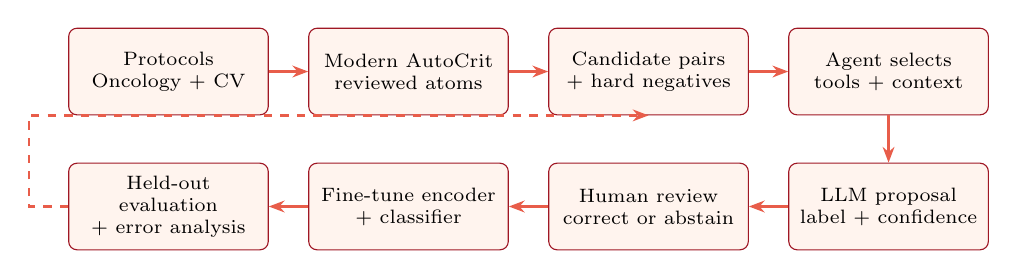
\begin{tikzpicture}[
  node distance=6mm and 5mm,
  box/.style={draw=wine,rounded corners=3pt,fill=cream,align=center,text width=23mm,minimum height=11mm,font=\scriptsize},
  arr/.style={-{Stealth[length=2mm]},thick,coral}
]
  \node[box] (p) {Protocols\\Oncology + CV};
  \node[box,right=of p] (m) {Modern AutoCrit\\reviewed atoms};
  \node[box,right=of m] (pair) {Candidate pairs\\+ hard negatives};
  \node[box,right=of pair] (agent) {Agent selects\\tools + context};
  \node[box,below=of agent] (llm) {LLM proposal\\label + confidence};
  \node[box,left=of llm] (human) {Human review\\correct or abstain};
  \node[box,left=of human] (train) {Fine-tune encoder\\+ classifier};
  \node[box,left=of train] (eval) {Held-out evaluation\\+ error analysis};
  \draw[arr] (p)--(m); \draw[arr] (m)--(pair); \draw[arr] (pair)--(agent);
  \draw[arr] (agent)--(llm); \draw[arr] (llm)--(human); \draw[arr] (human)--(train); \draw[arr] (train)--(eval);
  \draw[arr,dashed] (eval.west) -- ++(-5mm,0) |- (pair.south);
\end{tikzpicture}
\vspace{0.35cm}
\begin{block}{The agent powers the user workflow}
It retrieves protocol context and selects the appropriate comparison path. Explicit operators, intervals, and Boolean relations are evaluated with structured comparison tools; context-dependent clinical language is interpreted with embedding and LLM tools. The agent reconciles their evidence, records uncertainty, and escalates unresolved cases. Accepted corrections improve future versions of the tool.
\end{block}
\end{frame}

\begin{frame}{How a comparison is resolved}
\small
\begin{columns}[T,onlytextwidth]
  \column{0.31\textwidth}
  \begin{block}{1. Computable relation}
    \texttt{age $\geq 18$} versus \texttt{age $<18$}
    \begin{itemize}
      \item Parse operators and intervals
      \item Calculate overlap or disjointness
      \item Return an exact, inspectable result
    \end{itemize}
  \end{block}
  \column{0.31\textwidth}
  \begin{block}{2. Contextual relation}
    Cardiovascular history versus controlled hypertension
    \begin{itemize}
      \item Retrieve clinical context
      \item Use dense retrieval and LLM judgment
      \item Report rationale and uncertainty
    \end{itemize}
  \end{block}
  \column{0.31\textwidth}
  \begin{block}{3. Agent decision}
    \begin{itemize}
      \item Select one or both paths
      \item Check for conflicting evidence
      \item Accept, abstain, or request review
    \end{itemize}
  \end{block}
\end{columns}
\vspace{0.2cm}
\centering
\key{Human review is reserved for uncertain or conflicting cases—not every computable comparison.}
\end{frame}

\begin{frame}{How we will validate the tool}
\small
\begin{columns}[T,onlytextwidth]
  \column{0.48\textwidth}
  \key{Baselines and training}
  \begin{itemize}
    \item TF--IDF and frozen general/biomedical encoders
    \item Automated structured comparison where exact logic is available
    \item LLM judgment without fine-tuning
    \item Contrastive fine-tuning with positives, ordinary negatives, and hard negatives
    \item Directional classification head
  \end{itemize}
  \column{0.48\textwidth}
  \key{Evaluation}
  \begin{itemize}
    \item Protocol-level train/validation/test splits
    \item Retrieval recall@$k$ and ranking quality
    \item Macro-F1 and class-specific errors
    \item Calibration and input-order consistency
    \item Reviewer agreement, correction rate, and abstention quality
    \item Ablations of human corrections, critic, and structured checks
  \end{itemize}
\end{columns}
\vspace{0.1cm}
{\scriptsize\color{muted}Population comparisons, if feasible, use aggregate publication characteristics—not unavailable individual patient data or unsupported simulation.}
\end{frame}

\begin{frame}{From proposal to usable prototype}
\begin{columns}[T,onlytextwidth]
  \column{0.52\textwidth}
  \key{Build and validate}
  \begin{enumerate}
    \item Select comparable oncology and cardiovascular trials.
    \item Run and human-review Modern AutoCrit outputs.
    \item Freeze a versioned criterion dataset with provenance.
    \item Build diverse criterion pairs—not age alone.
    \item Run one frozen embedding baseline and identify failures.
    \item Train, calibrate, and test the agentic comparison pipeline.
  \end{enumerate}
  \column{0.44\textwidth}
  \key{User-facing prototype}
  \begin{itemize}
    \item Search or upload protocol criteria
    \item Retrieve comparable criteria across trials
    \item Show exact structured differences
    \item Classify clinical relationship
    \item Display confidence and rationale
    \item Escalate ambiguous cases to a reviewer
    \item Export reviewed comparisons for analysis
  \end{itemize}
\end{columns}
\end{frame}

\begin{frame}{Take-home message}
\begin{center}
  \Large
  \textcolor{wine}{\textbf{Modern AutoCrit structures what a protocol says.}}\\[5mm]
  \textcolor{coral}{\textbf{MetricSpace learns how criteria relate clinically.}}\\[7mm]
  \normalsize
  Protocol-centered \quad Agentic \quad Human-reviewed \quad Statistically validated
\end{center}
\vspace{0.6cm}
\begin{block}{Proposed deliverable}
A working clinical data-science application that extracts reviewed criteria, retrieves comparable rules across trials, explains their relationship, quantifies uncertainty, and preserves an audit trail—supported by a validated dense representation and agentic quality-control workflow.
\end{block}
\vfill
{\scriptsize\color{muted}
Starting references: Datta et al., \emph{AutoCriteria} (2023); Kury et al., \emph{Chia} (2020); Modern AutoCrit repository.}
\end{frame}

\end{document}
